\chapterimage{chapter_5.png}
\chapter{附录}

\begin{center}
    \pgfornament[width=0.36\linewidth,color=lsp]{88}
\end{center}

\section{比赛初始代码模板}
\lstinputlisting[style=cpp]{code/competition.cpp}

\section{unordered\_set/map 哈希函数}
\lstinputlisting[style=cpp]{code/hash.cpp}
写完自定义的哈希函数后,就可以通过 unordered\_map<int, int, my\_hash> my\_map; 或者 unordered\_map<pair<int, int>, int, my\_hash> my\_pair\_map; 的定义方式将自定义的哈希函数传入容器了。

\section{Big-O Cheat Sheet}

\subsection{Common Data Structure Operations}
\begin{figure}[H] %H为当前位置,!htb为忽略美学标准,htbp为浮动图形
\centering %图片居中
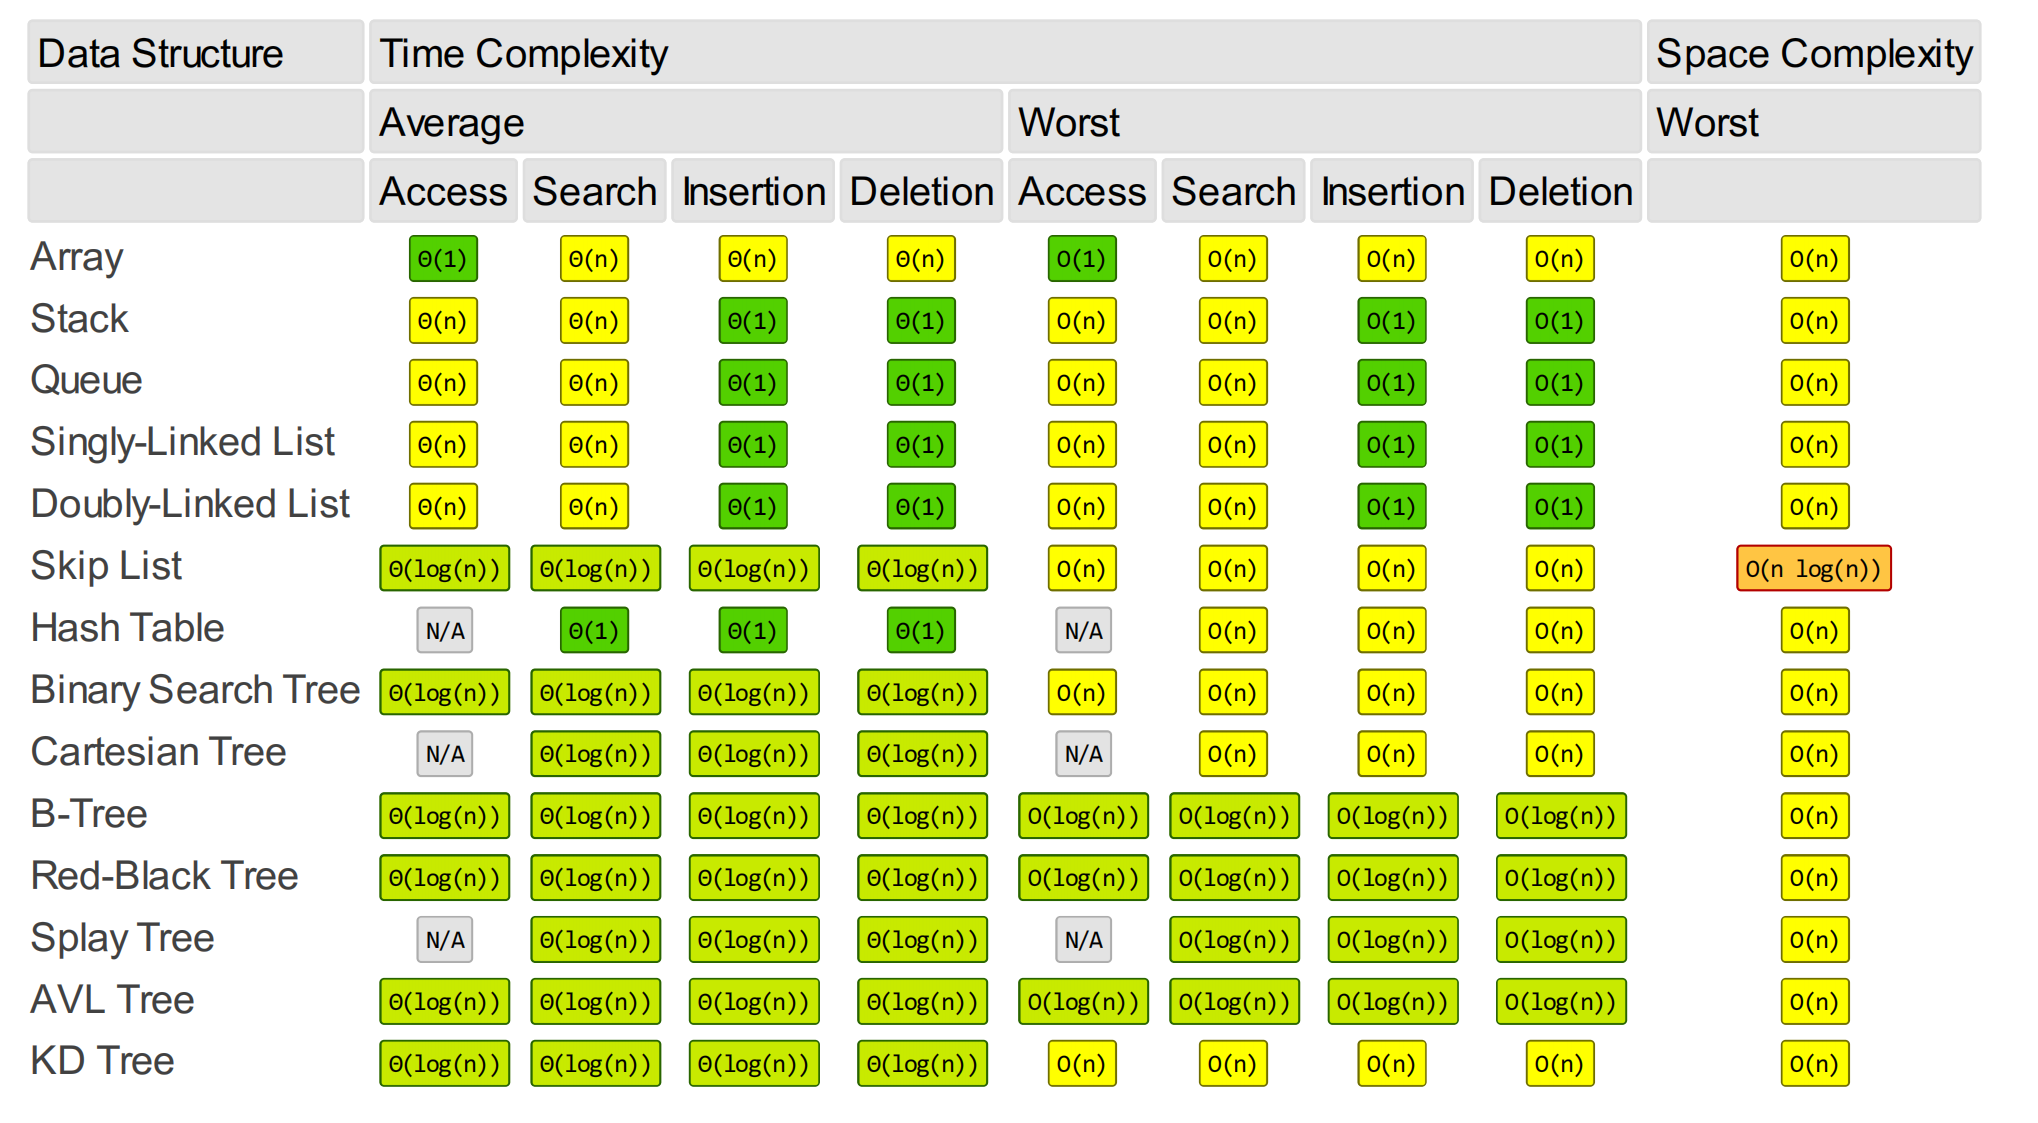
\includegraphics[width=0.9\textwidth]{images_content/1.png} %插入图片,[]中设置图片大小,{}中是图片文件名
\caption{Common Data Structure Operations} %最终文档中希望显示的图片标题
\end{figure}

\subsection{Array Sorting Algorithms}
\begin{figure}[H] %H为当前位置,!htb为忽略美学标准,htbp为浮动图形
\centering %图片居中
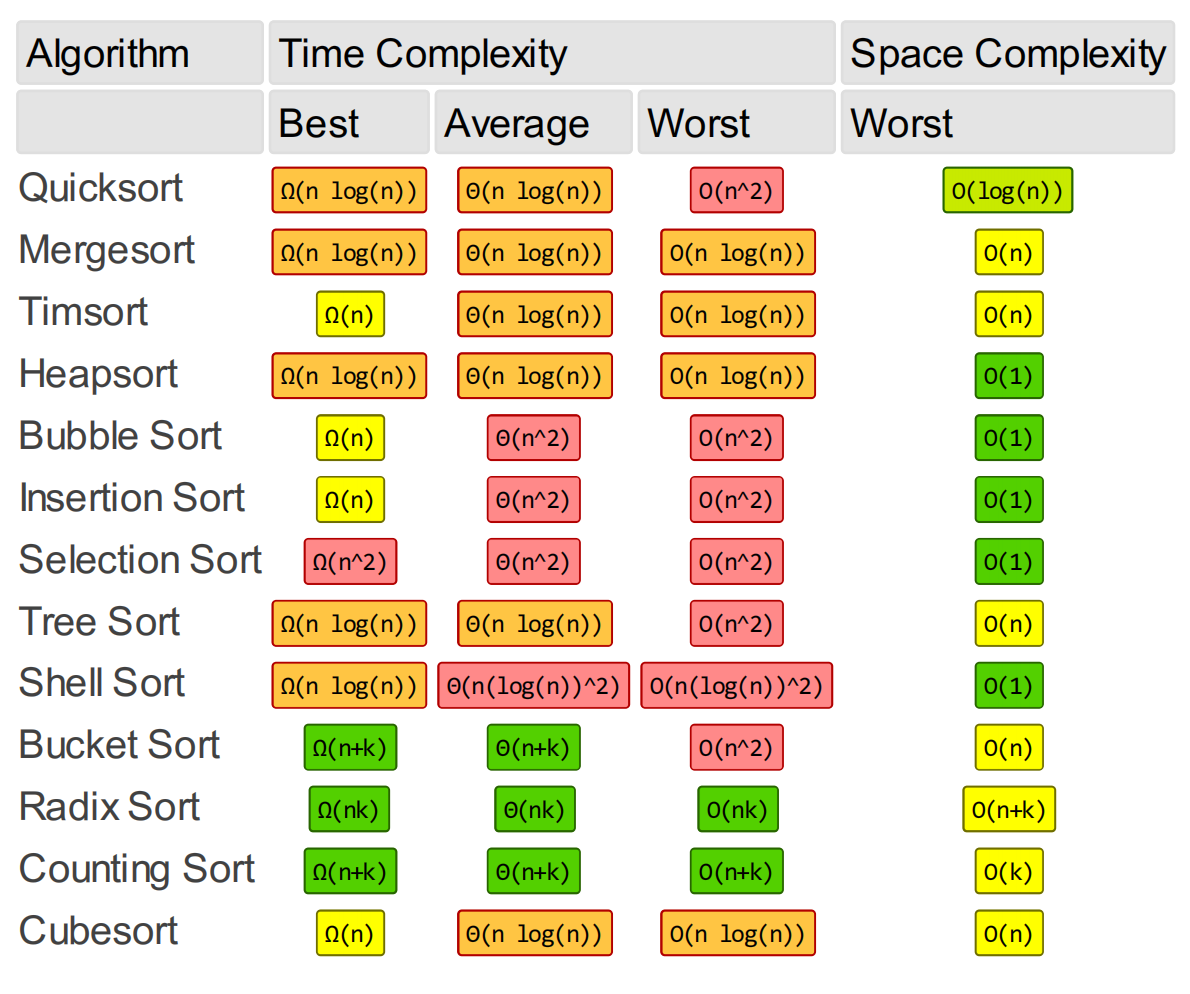
\includegraphics[width=0.7\textwidth]{images_content/2.png} %插入图片,[]中设置图片大小,{}中是图片文件名
\caption{Array Sorting Algorithms} %最终文档中希望显示的图片标题
\end{figure}

\subsection{Growth Rates}
\begin{figure}[H] %H为当前位置,!htb为忽略美学标准,htbp为浮动图形
\centering %图片居中
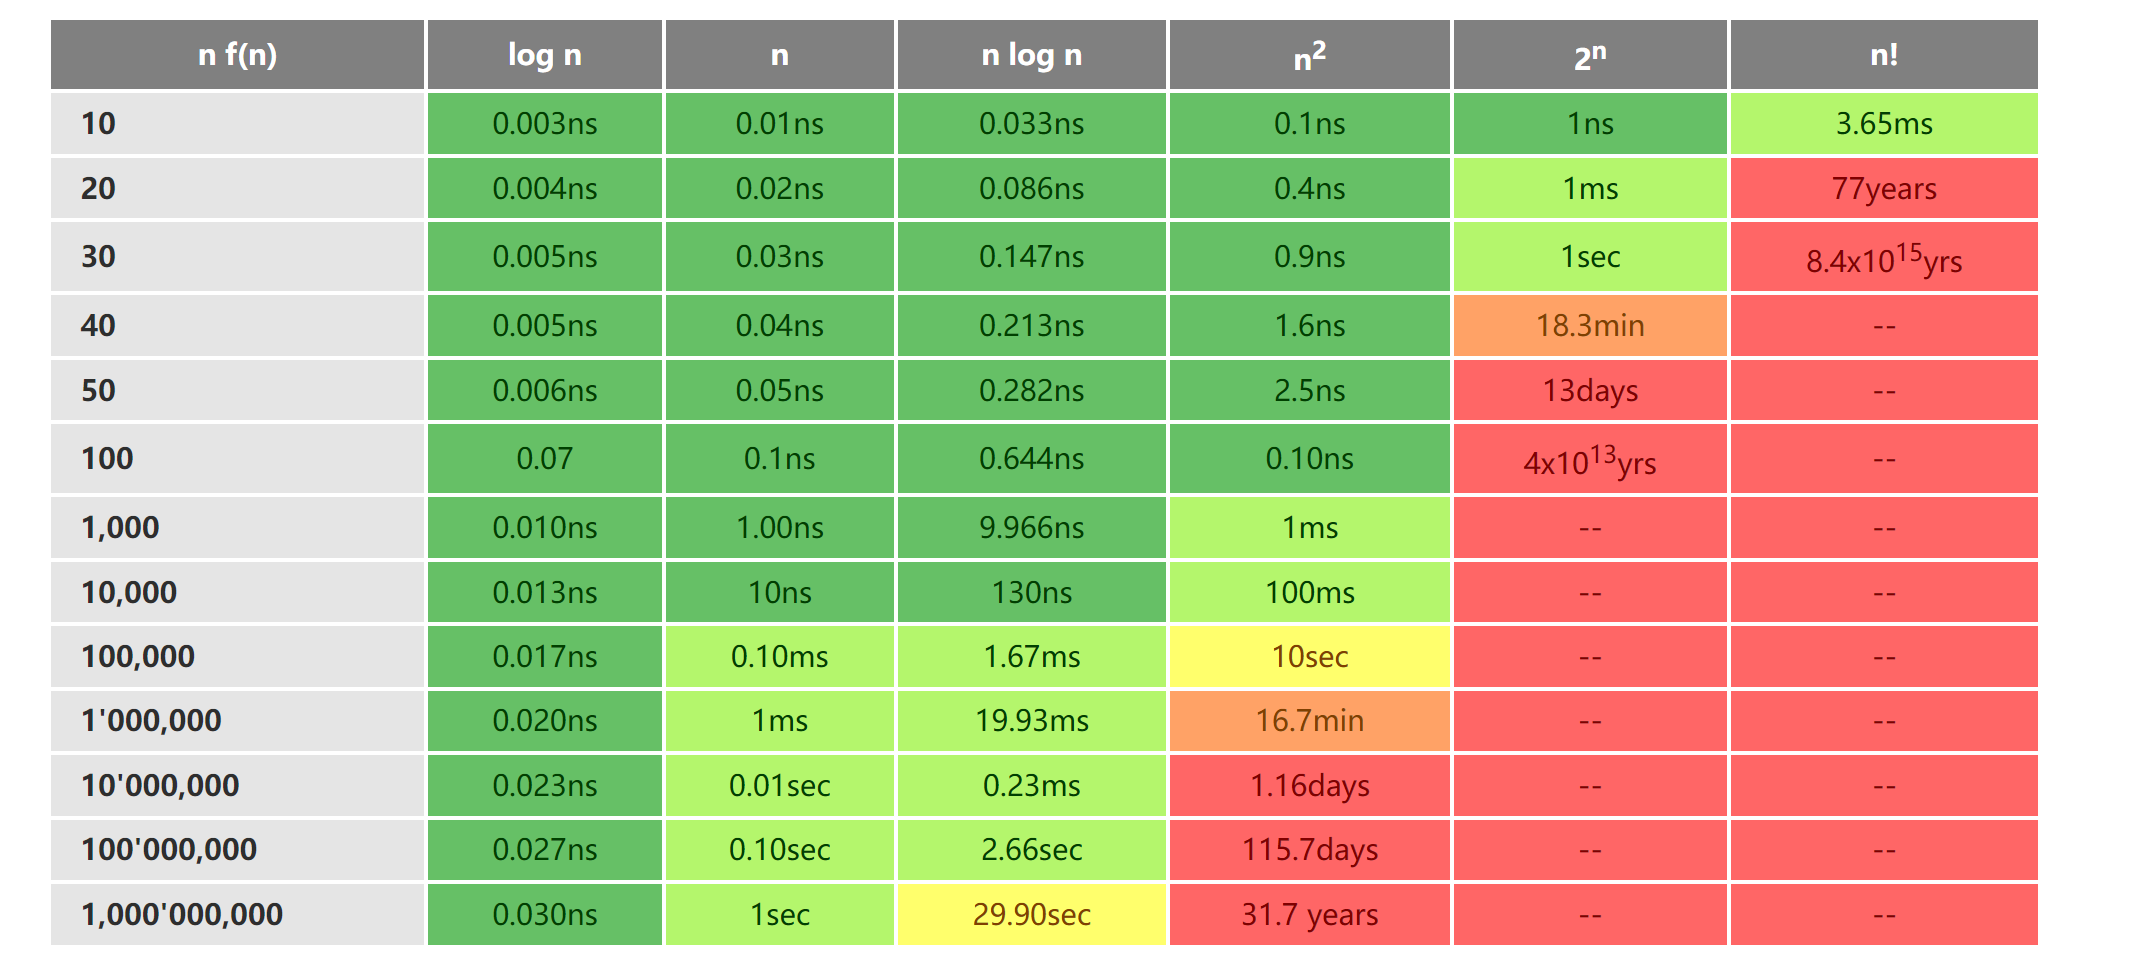
\includegraphics[width=0.9\textwidth]{images_content/3.png} %插入图片,[]中设置图片大小,{}中是图片文件名
\caption{Growth Rates} %最终文档中希望显示的图片标题
\end{figure}